%%%% 导言区
%% 设定纸张大小为A4, 基本字体大小为12pt, 文章题目单独为一页, 
%% 文档类型为article
\documentclass[a4paper,12pt]{article}

%% en_preamble包含基本的宏包配置
%%%%%%%%------------------------------------------------------------------------
%%%% 日常所用宏包

%% 控制页边距
\usepackage[top=2cm, bottom=2cm, left=2.cm, right=2.cm,includehead,includefoot]{geometry}

%% 控制项目列表
\usepackage{enumerate}

%% 多栏显示
\usepackage{multicol}

%% hyperref宏包,生成可定位点击的超链接,并且会生成pdf书签
\usepackage[%
    pdfstartview=FitH,%
    CJKbookmarks=true,%
    bookmarks=true,%
    bookmarksnumbered=true,%
    bookmarksopen=true,%
    colorlinks=true,%
    citecolor=blue,%
    linkcolor=blue,%
    anchorcolor=green,%
    urlcolor=blue%
]{hyperref}

%% 控制标题
\usepackage{titlesec}

%% 控制表格样式
\usepackage{booktabs}

%% 控制目录
\usepackage{titletoc}

%% 控制字体大小
\usepackage{type1cm}

%% 首行缩进,用\noindent取消某段缩进
\usepackage{indentfirst}

%% 支持彩色文本、底色、文本框等
\usepackage{color,xcolor}

%% AMS LaTeX宏包
\usepackage{amsmath}

%% 一些特殊符号
% \usepackage{bbding}

%% 支持引用
% \usepackage{cite}

%% LaTeX一些特殊符号宏包
% \usepackage{latexsym}

%% 数学公式中的黑斜体
% \usepackage{bm}

%% 调整公式字体大小:\mathsmaller, \mathlarger
% \usepackage{relsize}

%% 生成索引
% \makeindex

%%%% 基本插图方法
%% 图形宏包
\usepackage{graphicx}

%% 多个图形并排,参加lnotes.pdf
\usepackage{subfig}

% \begin{figure}[htbp]               %% 控制插图位置
%   \setlength{\abovecaptionskip}{0pt}
%   \setlength{\belowcaptionskip}{10pt}
                                     %% 控制图形和上下文的距离
%   \centering                       %% 使图形居中显示
%   \includegraphics[width=0.8\textwidth]{CTeXLive2008.jpg}
                                     %% 控制图形显示宽度为0.8\textwidth
%   \caption{CTeXLive2008安装过程} \label{fig:CTeXLive2008}
                                     %% 图形题目和交叉引用标签
% \end{figure}
%%%% 基本插图方法结束

%%%% pgf/tikz绘图宏包设置
\usepackage{pgf,tikz}
\usetikzlibrary{shapes,automata,snakes,backgrounds,arrows}
\usetikzlibrary{mindmap}
%% 可以直接在latex文档中使用graphviz/dot语言,
%% 也可以用dot2tex工具将dot文件转换成tex文件再include进来
%% \usepackage[shell,pgf,outputdir={docgraphs/}]{dot2texi}
%%%% pgf/tikz设置结束


%%%% fancyhdr设置页眉页脚
%% 页眉页脚宏包
\usepackage{fancyhdr}

%% 页眉页脚风格
\pagestyle{plain}

%% 有时会出现\headheight too small的warning
\setlength{\headheight}{15pt}

%% 清空当前页眉页脚的默认设置
%\fancyhf{}
%%%% fancyhdr设置结束


%%%% 设置listings宏包用来粘贴源代码
%% 方便粘贴源代码,部分代码高亮功能
\usepackage{listings}

%% 所要粘贴代码的编程语言
\lstloadlanguages{}

%% 设置listings宏包的一些全局样式
%% 参考http://hi.baidu.com/shawpinlee/blog/item/9ec431cbae28e41cbe09e6e4.html
\lstset{
showstringspaces=false,              %% 设定是否显示代码之间的空格符号
numbers=left,                        %% 在左边显示行号
numberstyle=\tiny,                   %% 设定行号字体的大小
basicstyle=\footnotesize,                    %% 设定字体大小\tiny, \small, \Large等等
keywordstyle=\color{blue!70}, commentstyle=\color{red!50!green!50!blue!50},
                                     %% 关键字高亮
frame=shadowbox,                     %% 给代码加框
rulesepcolor=\color{red!20!green!20!blue!20},
escapechar=`,                        %% 中文逃逸字符,用于中英混排
xleftmargin=2em,xrightmargin=2em, aboveskip=1em,
breaklines,                          %% 这条命令可以让LaTeX自动将长的代码行换行排版
extendedchars=false                  %% 这一条命令可以解决代码跨页时,章节标题,页眉等汉字不显示的问题
}
%%%% listings宏包设置结束


%%%% 附录设置
\usepackage[title,titletoc,header]{appendix}
%%%% 附录设置结束


%%%% 日常宏包设置结束
%%%%%%%%------------------------------------------------------------------------

%%%%%%%%------------------------------------------------------------------------
%%%% 英文字体设置结束
%% 这里可以加入自己的英文字体设置
%%%%%%%%------------------------------------------------------------------------

%%%%%%%%------------------------------------------------------------------------
%%%% 设置常用字体字号,与MS Word相对应

%% 一号, 1.4倍行距
\newcommand{\yihao}{\fontsize{26pt}{36pt}\selectfont}
%% 二号, 1.25倍行距
\newcommand{\erhao}{\fontsize{22pt}{28pt}\selectfont}
%% 小二, 单倍行距
\newcommand{\xiaoer}{\fontsize{18pt}{18pt}\selectfont}
%% 三号, 1.5倍行距
\newcommand{\sanhao}{\fontsize{16pt}{24pt}\selectfont}
%% 小三, 1.5倍行距
\newcommand{\xiaosan}{\fontsize{15pt}{22pt}\selectfont}
%% 四号, 1.5倍行距
\newcommand{\sihao}{\fontsize{14pt}{21pt}\selectfont}
%% 半四, 1.5倍行距
\newcommand{\bansi}{\fontsize{13pt}{19.5pt}\selectfont}
%% 小四, 1.5倍行距
\newcommand{\xiaosi}{\fontsize{12pt}{18pt}\selectfont}
%% 大五, 单倍行距
\newcommand{\dawu}{\fontsize{11pt}{11pt}\selectfont}
%% 五号, 单倍行距
\newcommand{\wuhao}{\fontsize{10.5pt}{10.5pt}\selectfont}
%%%%%%%%------------------------------------------------------------------------


%%%%%%%%------------------------------------------------------------------------
%%%% 一些个性设置

%% 设定页码方式,包括arabic、roman等方式
%% \pagenumbering{arabic}

%% 有时LaTeX无从断行,产生overfull的错误,这条命令降低LaTeX断行标准
%% \sloppy

%% 设定目录显示深度\tableofcontents
%% \setcounter{tocdepth}{2}
%% 设定\listoftables显示深度
%% \setcounter{lotdepth}{2}
%% 设定\listoffigures显示深度
%% \setcounter{lofdepth}{2}

%% 设定段间距
\setlength{\parskip}{0.3\baselineskip}

%% 设定行距
\linespread{1}

%% 中文破折号,据说来自清华模板
\newcommand{\pozhehao}{\kern0.3ex\rule[0.8ex]{2em}{0.1ex}\kern0.3ex}

%% 设定itemize环境item的符号
\renewcommand{\labelitemi}{$\bullet$}

%% 设定正文字体大小
% \renewcommand{\normalsize}{\sihao}

%%%% 个性设置结束
%%%%%%%%------------------------------------------------------------------------


%%%%%%%%------------------------------------------------------------------------
%%%% bibtex设置

%% 设定参考文献显示风格
\bibliographystyle{unsrt}

%%%% bibtex设置结束
%%%%%%%%------------------------------------------------------------------------


%% 如果不写中文的话就不需要引用xecjk_preamble里面的配置
%%%%%%%%------------------------------------------------------------------------
%%%% xeCJK相关宏包

\usepackage{xltxtra,fontspec,xunicode}

%% \CJKsetecglue{\hskip 0.15em plus 0.05em minus 0.05em}
%% slanfont: 允许斜体
%% boldfont: 允许粗体
%% CJKnormalspaces: 仅忽略汉字之间的空白,但保留中英文之间的空白。 
%% CJKchecksingle: 避免单个汉字单独占一行。
\usepackage[slantfont, boldfont]{xeCJK} 

%% 针对中文进行断行
\XeTeXlinebreaklocale "zh"             

%% 给予TeX断行一定自由度
\XeTeXlinebreakskip = 0pt plus 1pt minus 0.1pt

%%%% xeCJK设置结束                                       
%%%%%%%%------------------------------------------------------------------------

%%%%%%%%------------------------------------------------------------------------
%%%% xeCJK字体设置

%% 设置中文标点样式,支持quanjiao、banjiao、kaiming等多种方式
\punctstyle{kaiming}                                        

%% 设置缺省中文字体
\setCJKmainfont[BoldFont={FandolHei}, ItalicFont={FandolKai}]{SimSun}   
%% 设置中文无衬线字体
\setCJKsansfont[BoldFont={FandolHei}]{FandolKai}  
%% 设置等宽字体
\setCJKmonofont{FandolHei}                             

%% 英文衬线字体
\setmainfont{DejaVu Serif}                                  
%% 英文等宽字体
\setmonofont{DejaVu Sans Mono}                              
%% 英文无衬线字体
\setsansfont{DejaVu Sans}                                   

%% 定义新字体
\setCJKfamilyfont{song}{SimSun}                     
\setCJKfamilyfont{kai}{SimSun}
\setCJKfamilyfont{hei}{FandolHei}
\setCJKfamilyfont{FandolFang}{}
%\setCJKfamilyfont{lisu}{LiSu}
%\setCJKfamilyfont{youyuan}{YouYuan}

%% 自定义宋体
\newcommand{\song}{\CJKfamily{song}}                       
%% 自定义楷体
\newcommand{\kai}{\CJKfamily{kai}}                         
%% 自定义黑体
\newcommand{\hei}{\CJKfamily{hei}}                         
%% 自定义仿宋体
\newcommand{\fangsong}{\CJKfamily{fangsong}}               
%% 自定义隶书
%\newcommand{\lisu}{\CJKfamily{lisu}}                       
%% 自定义幼圆
%\newcommand{\youyuan}{\CJKfamily{youyuan}}                 

%%%% xeCJK字体设置结束
%%%%%%%%------------------------------------------------------------------------

%%%%%%%%------------------------------------------------------------------------
%%%% 一些关于中文文档的重定义

%% 数学公式定理的重定义

\newtheorem{example}{例}                                   
\newtheorem{algorithm}{算法}
%% 按section编号
\newtheorem{theorem}{定理}[section]                         
\newtheorem{definition}{定义}
\newtheorem{axiom}{公理}
\newtheorem{property}{性质}
\newtheorem{proposition}{命题}
\newtheorem{lemma}{引理}
\newtheorem{corollary}{推论}
\newtheorem{remark}{注解}
\newtheorem{condition}{条件}
\newtheorem{conclusion}{结论}
\newtheorem{assumption}{假设}

%% 章节等名称重定义
\renewcommand{\contentsname}{目\hspace{1.5cm}录}     
\renewcommand{\abstractname}{摘要}
\renewcommand{\indexname}{索引}
\renewcommand{\listfigurename}{插图目录}
\renewcommand{\listtablename}{表格目录}
\renewcommand{\figurename}{图}
\renewcommand{\tablename}{表}
\renewcommand{\appendixname}{附录}
\renewcommand{\appendixpagename}{附录}
\renewcommand{\appendixtocname}{附录}
\renewcommand\refname{参考文献} 

%% 设置chapter、section与subsection的格式
\titleformat{\chapter}{\centering\huge}{第\thechapter{}章}{1em}{\textbf}
%\titleformat{\section}{\centering\sanhao}{\hei \biaotiNR\thesection}{1em}{\textbf}
%\titleformat{\subsection}{\xiaosi}{\thesubsection}{1em}{\textbf}
%\titleformat{\subsubsection}{\xiaosi}{\thesubsubsection}{1em}{\textbf}

%%%% 中文重定义结束
%%%%%%%%------------------------------------------------------------------------


%% 首页格式
\usepackage{tabu} % 用tabu代替 array
\usepackage{multirow}
\usepackage{zhnumber}
\usepackage{calc,marvosym,ifthen,fancybox,url,layout}
\setcounter{tocdepth}{1}

%设定标题
\setcounter{secnumdepth}{5}
\titleformat{\section}{\centering\sanhao}{\hei \biaotiNR\thesection}{1em}{\hei}
\titleformat{\subsection}{\xiaosi}{\hskip -2pt \Roman{subsection}}{1em}{\hei}
\titleformat{\subsubsection}{\xiaosi}{\hei\zhnumber{\arabic{subsubsection}}、}{1em}{\textbf}
\titleformat{\paragraph}{\xiaosi}{\arabic{paragraph}、}{1em}{}
\titleformat{\subparagraph}{\xiaosi}{(\arabic{subparagraph})}{1em}{}
%调整标题间距
\titlespacing{\subsection}{0pt}{*0}{*0}
\titlespacing{\subsubsection}{0pt}{*0}{*0}
\titlespacing{\section}{0pt}{*0}{*0}
\titlespacing{\paragraph}{0pt}{*0}{*0}
\titlespacing{\subparagraph}{0pt}{*0}{*0}
 
 %给旁注加个黑原点
\usepackage{wasysym}
\let\marginparNR\marginpar
\def\marginpar#1{\marginparNR{ \CIRCLE{}   #1  }}

%调整列表前后的间距
\makeatletter
\let\orig@Enumerate=\enumerate
\renewenvironment{enumerate}{\orig@Enumerate}{\vspace{-0.5cm}\endlist}
\let\orig@Itemize=\itemize
\renewenvironment{itemize}{\orig@Itemize}{\vspace{-0.5cm}\endlist}
\makeatother

%给目录进行设定
\titlecontents{section}[0pt]{\addvspace{5pt}\filright}
{ \biaotiNR \thecontentslabel \hspace{0.5em} }
{}{\titlerule*[8pt]{.}\contentspage}


%画边框
%\def\boxhack{\leavevmode\vbox to0pt{\vss\rlap{\hskip 320pt
%			\setlength{\unitlength}{1pt}\cornersize*{10pt}\thicklines\fancyoval(365,675)}\vskip -680pt}}
%\def\boxhackb{\leavevmode\vbox to0pt{\vss\rlap{\hskip 80pt
%			\setlength{\unitlength}{1pt}\cornersize*{10pt}\thicklines\fancyoval(100,675)}\vskip -680pt}}

%用tikz画边框	
\def\biankuang{\leavevmode\vbox to0pt{
		\vss\rlap{\hskip 0.8cm
			\tikz \draw(4,0)--(0,0)--(0,-23.7)--(16.7,-23.7)--(16.7,0)--(4,0)--(4,-23.7);		
		}\vskip -24cm}}
		
\newcolumntype{M}[1]{>{\sihao\centering\arraybackslash}m{#1}}
\newcolumntype{N}{@{}m{0pt}@{}}

\newcommand{\ktmq}[1]{\gdef\ktmqNR{#1}}%课题名称
\newcommand{\jxmb}[1]{\gdef\jxmbNR{#1}}%教学目标
\newcommand{\jxnd}[1]{\gdef\jxndNR{#1}}%教学难点
\newcommand{\jxzd}[1]{\gdef\jxzdNR{#1}}%教学重点
\newcommand{\jjff}[1]{\gdef\jjffNR{#1}}%解决方法
\newcommand{\jxhj}[1]{\gdef\jxhjNR{#1}}%教学后记

\newcommand{\jc}[1]{\gdef\jcNR{#1}}%教材
\newcommand{\cks}[1]{\gdef\cksNR{#1}}%参考书
\newcommand{\jsxm}[1]{\gdef\jsxmNR{#1}}%教师姓名
\newcommand{\jyszr}[1]{\gdef\jyszrNR{#1}}%教研室主任

\newcommand{\skbc}[1]{\gdef\skbcNR{#1}}%授课班次
\newcommand{\skrq}[1]{\gdef\skrqNR{#1}}%授课日期
\newcommand{\biaoti}[1]{\gdef\biaotiNR{#1}}%标题头

\newcounter{thesectionSY}

\newcommand{\makeshouye}{
	\setcounter{thesectionSY}{\thesection+1}
	\restoregeometry	
	\renewcommand{\headrulewidth}{0pt}
	\pagestyle{fancy}
	\fancyhead{}
	\lhead{} 
	\chead{
		\begin{tabular}{@{\hspace{1.2cm}}M{7cm}@{\hspace{-0.4cm}}M{8cm}N}
			\parbox{7cm}{\linespread{0.2}
				\makebox[7cm][s]{\kai \sanhao 湖南九嶷职业技术学院}\\ 
				\makebox[7cm][s]{\kai \sanhao 湖南潇湘技师学院}
			}
			&  \makebox[6cm][s]{\rule{0pt}{0.9cm}\yihao \hei 授课课时计划}\\
		\end{tabular}
	}
	
	\begin{tabular}{M{2.2cm}|M{7cm}|M{5.8cm}N}
		\hline
		\multirow{2}*{
			\rule{0pt}{1.4cm}\parbox[b]{2.cm}{
				\centering 课\hfill 程\hfill 章\hfill 节\\及\hfill 主\hfill 题}}& \hei \biaotiNR\thethesectionSY  &  ~授~课~教~师\hfill {\kai \sanhao \underline{\jsxmNR}}\hfill 签字~~~&\\[0.6cm] \cline{2-3}
		
		& \hei \ktmqNR &  ~教研室主任\hfill {\fangsong \sanhao \underline{\jyszrNR}}\hfill 签字~~~&\\[0.6cm]\hline
		
		\multicolumn{3}{l}{
			\begin{minipage}[t][4cm][t]{15cm}	
				\begin{minipage}[t]{2.5cm}
					\vspace{6pt} \hfill \sihao 教学目标:
				\end{minipage}\hspace{0.5cm}				
				\begin{minipage}[t][4cm][t]{12cm}
					\vspace{0pt}\sihao \setlength{\baselineskip}{12pt} 
					\begin{enumerate}[1、]
						\jxmbNR
					\end{enumerate} 
				\end{minipage} 
			\end{minipage}
		}\vspace{0.3cm} &\\ \hline
		\multicolumn{3}{l}{
			\begin{minipage}[t][6.5cm][t]{15cm}
				\begin{minipage}[t]{2.5cm}
					\vspace{5pt} \hfill \sihao 教学重点:
				\end{minipage}\hspace{0.5cm}				
				\begin{minipage}[t]{12cm}
					\vspace{0pt} \sihao \setlength{\baselineskip}{12pt} 
					\begin{enumerate}[1、] \jxzdNR \end{enumerate}
					\vspace{7pt} 
				\end{minipage}
				\vspace{5pt} 
				\begin{minipage}[t]{2.5cm}
					\vspace{6pt} \hfill \sihao 教学难点:
				\end{minipage}\hspace{0.5cm}		
				\begin{minipage}[t]{12cm}
					\vspace{0pt} \sihao \setlength{\baselineskip}{12pt} 
					\begin{enumerate}[1、] \jxndNR \end{enumerate}
					\vspace{0pt} 	
				\end{minipage}
				\begin{minipage}[t]{2.5cm}
					\vspace{6pt} \hfill \sihao 解决方法:
				\end{minipage}\hspace{0.5cm}		
				\begin{minipage}[t]{12cm}
					\vspace{6pt}\sihao \jjffNR
				\end{minipage}
				
			\end{minipage}
		} &\\  \hline
		
		\multirow{2}*{ 	\rule{0pt}{1.4cm}\parbox[b]{2.cm}{
				\centering 教\hfill 材\hfill 和\\参\hfill 考\hfill 书 } } & \multicolumn{2}{c}{\sihao \jcNR } &\\[0.6cm] \cline{2-3}
		&  \multicolumn{2}{c}{\sihao \cksNR } &\\[0.6cm] \hline
		\multirow{2}*{\rule{0pt}{1.4cm}\parbox[b]{2.cm}{
				\centering 授\hfill 课\hfill 班\hfill 次\\授\hfill 课\hfill 日\hfill 期 } } & \multicolumn{2}{c}{ \skbcNR } &\\[0.6cm] \cline{2-3}
		&\multicolumn{2}{c}{ \skrqNR } &\\[0.6cm] \hline
		
		\multicolumn{3}{l}{
			\begin{minipage}[t]{2.5cm}
				\vspace{0pt} \hfill \sihao 教学后记:
			\end{minipage}\hspace{0.5cm}				
			\begin{minipage}[t][4.5cm][t]{12cm}
				\vspace{0pt}\sihao \jxhjNR
			\end{minipage} 
		}\vspace{0.3cm} &\\ \hline	
	\end{tabular}
	\newpage
\newgeometry{textwidth={\textwidth-150pt},top=2cm,bottom=2cm,right=2.5cm,includehead,includefoot,marginparsep=28pt,marginparwidth=85pt}
	
\reversemarginpar
\fancyhead{} 
\chead{\kai \yihao 教 \hspace{1cm} 案 \hspace{1cm} 纸 }
%\lhead{\boxhack \boxhackb } %边框 
\lhead{ \biankuang}%边框 
		
\section{ \ktmqNR }
}



%%%% 导言区结束
%%%%%%%%------------------------------------------------------------------------

%%%%%%%%------------------------------------------------------------------------

%%%% 公共信息
\jsxm{高老师} %教师姓名
\jyszr{高星}	%教研室主任
\jc{《加工中心编程与操作》刘加孝主编}%教材
\cks{}%参考书
\skbc{15级中数班}%授课班次
\biaoti{理论}%标题头

%%%% 正文部分
\begin{document}

\begin{titlepage}

\begin{center}
{ \yihao \bf
\makebox[10cm][s]{湖南九嶷职业技术学院}  \\
\makebox[10cm][s]{湖南潇湘技师学院} \\ }
\vfill 
{ \yihao \fangsong  \fontsize{46pt}{80pt}\selectfont
   教
\par 案
\par 本
\par }
\par
\vfill \vfill \sihao \setlength{\baselineskip}{1cm}  \bf  
 授课教师:\underline{ \makebox[5cm]{ \jsxmNR}}\par
 授课课程:\underline{ \makebox[5cm]{ 数铣编程与操作}}\par
授课班级:\underline{ \makebox[5cm]{ \skbcNR}} 
\vfill
{\bf 二O一六 }——{\bf 二O一七}学年\hspace{0.5cm} 第{\bf 二}学期
\end{center}
\vfill
\end{titlepage}


\tableofcontents
\setcounter{page}{-0}
\thispagestyle{empty}

\jxhj{%教学后记
	}
\skrq{%授课日期
	}
\ktmq{%课题名称
	复习上期所学内容 }
\jxmb{%教学目标,每行前面要加 \item
	\item 巩固上期的基本指令;

	\item 总结上期的编程思路;

	\item 总结机床的操作技巧;

	\item 了解本期的学习内容及学生情况;}
\jxzd{%教学重点,每行前面要加 \item
	\item 巩固上期的基本指令;

	\item 总结上期的编程思路;}
\jxnd{%教学难点,每行前面要加 \item
	\item 总结上期的编程思路;}
\jjff{%教学方法
	通过讲述、举例、演示法来说明;}

\makeshouye %制作教案首页

%%%%教学内容
\subsection{组织教学}
\begin{enumerate}[\hspace{2em}1、]
	\setlength{\itemsep}{0pt}
	\item 集中学生注意力;
	\item 清查学生人数;
	\item 维持课堂纪律;
\end{enumerate}
\subsection{复习导入及主要内容}
\begin{enumerate}[\hspace{2em}1、]
	\item 上学期末考试讲评;

	\item 了解学生情况;
\end{enumerate}
\subsection{教学内容及过程}
\subsubsection{本期教学安排} \marginpar{说明介绍}
\paragraph{理论教学计划:}
\begin{itemize}
	\item 复习上期内容

	\item 两面加工实例

	\item 变量与基本运算

	\item 椭圆加工if  goto

	\item 循环及其指令 if goto while

	\item 循环应用

	\item Siemens参数编程概述

	\item Siemens应用

	\item 镜象指令的使用

	\item 薄壁及配合件加工工艺

	\item 双曲线、抛物线加工

	\item 孔系加工(循环嵌套)

	\item 圆孔的宏程序

	\item 方槽椭圆槽的宏程序
	\item 斜面与圆柱面的宏程序

	\item 球面的宏程序(凸/凹)

	\item 椭球面的宏程序

	\item 任意轮廓倒圆角(系统变量)

	\item 任意轮廓倒圆角(G10)

	\item Siemens上倒角与倒圆

	\item 宏程序调用基本知识

	\item 宏程序调用的应用

	\item 多轴加工概述

	\item 四轴加工:圆柱凸轮的加工

	\item 五轴加工简介

	\item 综合练习(一)

	\item 综合练习(二)

	\item 综合练习(三)

	\item 综合练习(四)

\end{itemize}

\paragraph{实习教学计划}
\begin{itemize}
	\item 两面加工类零件加工

	\item 薄壁配合件加工

	\item 宏程序加工

	\item 综合加工(钢材)
\end{itemize}

\subsubsection{手工编程复习} \marginpar{互动提问}
如下面的思维导图 \ref{手工编程思维导图}
\begin{figure}	
	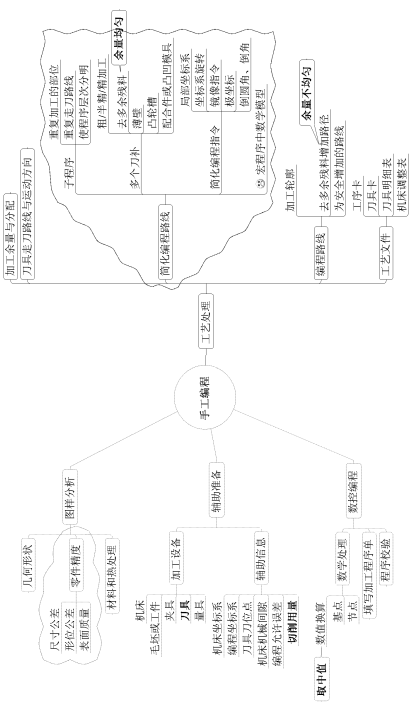
\includegraphics{images/图片1} 
	\caption{手工编程思维导图}\label{手工编程思维导图}
\end{figure}

\subsubsection{数控机床的操作}
如下面的思维导图 \ref{数控机床的操作思维导}
\begin{figure}	
	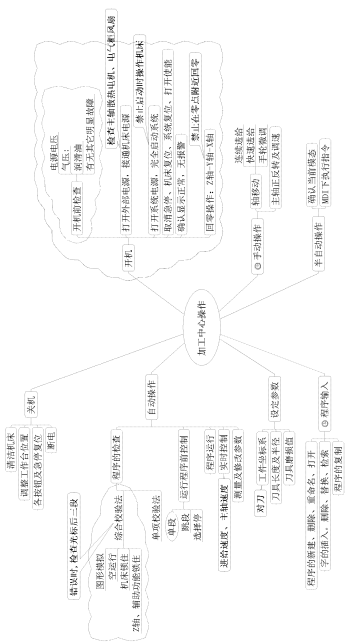
\includegraphics{images/图片2} 
	\caption{数控机床的操作思维导图} \label{数控机床的操作思维导}
\end{figure}

\subsubsection{数控机床指令}
\paragraph{G指令}\begin{itemize}
	\item G0 G1 G2 G3

	\item G17 G18 G19

	\item G9 G61 G62 G63 G64

	\item G4 \marginpar{说明介绍说明介绍说明介绍说明介绍说明介绍说明介绍}

	\item G20 G21

	\item G40 G41 G42 

	\item G43 G44 G49 \marginpar{说明介绍说明介绍说明介绍说明介绍说明介绍说明介绍}

	\item G90 G91

	\item G98 G99

	\item G81 G82 G83 G84 G85 G86 G87 G88 G89 G80 G73 G74 G76

\end{itemize}

\paragraph{M指令}

\begin{itemize}
	\item M0 M1 M2 M30

	\item M3 M4 M5 M19 

	\item M6 M7 M8 M9

	\item M98 M99

\end{itemize}

\paragraph{其它指令}
\subsubsection{常见加工结构}
\begin{itemize}
	\item 平面

	\item 外轮廓

	\item (岛屿)

	\item 孔
	\item 凸轮槽

	\item 复杂零件

	\item 配合零件

	\item CAD/CAM

	\item 宏程序

	\item 其它
\end{itemize}
\subsubsection{上学期期末试卷分析}
\subsection{课堂小结}
主要复习了数控方面的基本知识。
\vfill
\subsection{布置作业}
\begin{enumerate}[1、]
	\item 自选一零件图, 写出其工艺与程序;

	\item 写出如图所示零件的程序及与工艺;
\end{enumerate}


\jxhj{%教学后记
	}
\skrq{%授课日期
	}
\ktmq{%课题名称
	学习新内容 }
\jxmb{%教学目标,每行前面要加 \item
	\item 巩固上期的基本指令;

	\item 总结上期的编程思路;

	\item 总结机床的操作技巧;

	\item 了解本期的学习内容及学生情况;}
\jxzd{%教学重点,每行前面要加 \item
	\item 巩固上期的基本指令;

	\item 总结上期的编程思路;}
\jxnd{%教学难点,每行前面要加 \item
	\item 总结上期的编程思路;}
\jjff{%教学方法
	通过讲述、举例、演示法来说明;}

\makeshouye %制作教案首页

%%%%教学内容
\subsection{组织教学}
\begin{enumerate}[\hspace{2em}1、]
	\item 集中学生注意力;
	\item 清查学生人数;
	\item 维持课堂纪律;
\end{enumerate}
\subsection{复习导入及主要内容}
\begin{enumerate}[\hspace{2em}1、]
	\item 上学期末考试讲评;

	\item 了解学生情况;
\end{enumerate}
\subsection{教学内容及过程}
\subsubsection{本期教学安排} \marginpar{说明介绍}
\paragraph{理论教学计划:}
\begin{itemize}
	\item 复习上期内容

	\item 两面加工实例

	\item 变量与基本运算

	\item 椭圆加工if  goto

	\item 循环及其指令 if goto while

	\item 循环应用

	\item Siemens参数编程概述

	\item Siemens应用

	\item 镜象指令的使用

	\item 薄壁及配合件加工工艺

	\item 双曲线、抛物线加工

	\item 孔系加工(循环嵌套)

	\item 圆孔的宏程序

	\item 方槽椭圆槽的宏程序
	\item 斜面与圆柱面的宏程序

	\item 球面的宏程序(凸/凹)

	\item 椭球面的宏程序

	\item 任意轮廓倒圆角(系统变量)

	\item 任意轮廓倒圆角(G10)

	\item Siemens上倒角与倒圆

	\item 宏程序调用基本知识

	\item 宏程序调用的应用

	\item 多轴加工概述

	\item 四轴加工:圆柱凸轮的加工

	\item 五轴加工简介

	\item 综合练习(一)

	\item 综合练习(二)

	\item 综合练习(三)

	\item 综合练习(四)

\end{itemize}

\subparagraph{实习教学计划}
\begin{itemize}
	\item 两面加工类零件加工

	\item 薄壁配合件加工

	\item 宏程序加工

	\item 综合加工(钢材)
\end{itemize}

\subsubsection{手工编程复习} \marginpar{互动提问}
如下面的思维导图 \ref{手工编程思维导图}
\begin{figure}	
	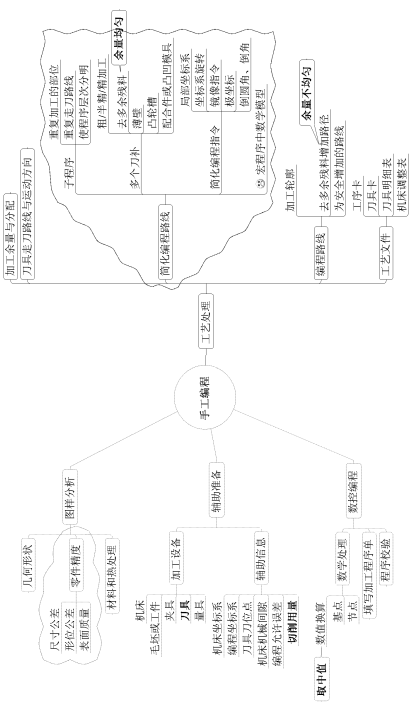
\includegraphics{images/图片1} 
	\caption{手工编程思维导图}\label{手工编程思维导图}
\end{figure}

\subsubsection{数控机床的操作}
如下面的思维导图 \ref{数控机床的操作思维导}
\begin{figure}	
	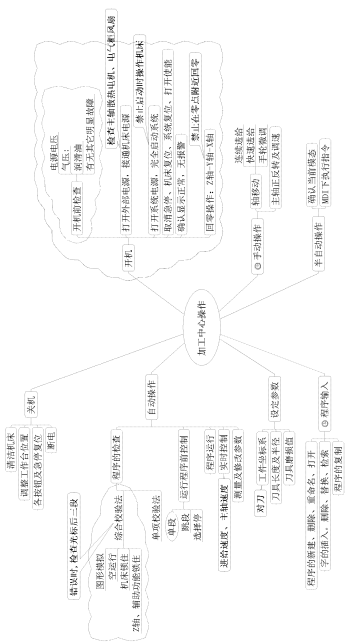
\includegraphics{images/图片2} 
	\caption{数控机床的操作思维导图} \label{数控机床的操作思维导}
\end{figure}

\subsubsection{数控机床指令}
\paragraph{G指令}\begin{itemize}
	\item G0 G1 G2 G3

	\item G17 G18 G19

	\item G9 G61 G62 G63 G64

	\item G4 

	\item G20 G21

	\item G40 G41 G42 

	\item G43 G44 G49

	\item G90 G91

	\item G98 G99

	\item G81 G82 G83 G84 G85 G86 G87 G88 G89 G80 G73 G74 G76

\end{itemize}

\paragraph{M指令}

\begin{itemize}
	\item M0 M1 M2 M30

	\item M3 M4 M5 M19

	\item M6 M7 M8 M9

	\item M98 M99

\end{itemize}

\paragraph{其它指令}
\subsubsection{常见加工结构}
\begin{itemize}
	\item 平面

	\item 外轮廓

	\item (岛屿)

	\item 孔
	\item 凸轮槽

	\item 复杂零件

	\item 配合零件

	\item CAD/CAM

	\item 宏程序

	\item 其它
\end{itemize}
\subsubsection{上学期期末试卷分析}
\subsection{课堂小结}
主要复习了数控方面的基本知识。
\vfill
\subsection{布置作业}
\begin{enumerate}[1、]
	\item 自选一零件图, 写出其工艺与程序.

	\item 写出如图所示零件的程序及与工艺.
\end{enumerate}


\biaoti{实习}%标题头
\setcounter{section}{0}%重新计数
%重新设定目录
\titlecontents{section}[0pt]{\addvspace{5pt}\filright}
{ 实习  \thecontentslabel \hspace{0.5em} }
{}{\titlerule*[8pt]{.} \contentspage}
\jxhj{%教学后记
	}
\skrq{%授课日期
	}
\ktmq{%课题名称
	复习上期所学内容 }
\jxmb{%教学目标,每行前面要加 \item
	\item 巩固上期的基本指令;

	\item 总结上期的编程思路;

	\item 总结机床的操作技巧;

	\item 了解本期的学习内容及学生情况;}
\jxzd{%教学重点,每行前面要加 \item
	\item 巩固上期的基本指令;

	\item 总结上期的编程思路;}
\jxnd{%教学难点,每行前面要加 \item
	\item 总结上期的编程思路;}
\jjff{%教学方法
	通过讲述、举例、演示法来说明;}

\makeshouye %制作教案首页

%%%%教学内容
\subsection{组织教学}
\begin{enumerate}[\hspace{2em}1、]
	\setlength{\itemsep}{0pt}
	\item 集中学生注意力;
	\item 清查学生人数;
	\item 维持课堂纪律;
\end{enumerate}
\subsection{复习导入及主要内容}
\begin{enumerate}[\hspace{2em}1、]
	\item 上学期末考试讲评;

	\item 了解学生情况;
\end{enumerate}
\subsection{教学内容及过程}
\subsubsection{本期教学安排} \marginpar{说明介绍}
\paragraph{理论教学计划:}
\begin{itemize}
	\item 复习上期内容

	\item 两面加工实例

	\item 变量与基本运算

	\item 椭圆加工if  goto

	\item 循环及其指令 if goto while

	\item 循环应用

	\item Siemens参数编程概述

	\item Siemens应用

	\item 镜象指令的使用

	\item 薄壁及配合件加工工艺

	\item 双曲线、抛物线加工

	\item 孔系加工(循环嵌套)

	\item 圆孔的宏程序

	\item 方槽椭圆槽的宏程序
	\item 斜面与圆柱面的宏程序

	\item 球面的宏程序(凸/凹)

	\item 椭球面的宏程序

	\item 任意轮廓倒圆角(系统变量)

	\item 任意轮廓倒圆角(G10)

	\item Siemens上倒角与倒圆

	\item 宏程序调用基本知识

	\item 宏程序调用的应用

	\item 多轴加工概述

	\item 四轴加工:圆柱凸轮的加工

	\item 五轴加工简介

	\item 综合练习(一)

	\item 综合练习(二)

	\item 综合练习(三)

	\item 综合练习(四)

\end{itemize}

\paragraph{实习教学计划}
\begin{itemize}
	\item 两面加工类零件加工

	\item 薄壁配合件加工

	\item 宏程序加工

	\item 综合加工(钢材)
\end{itemize}

\subsubsection{手工编程复习} \marginpar{互动提问}
如下面的思维导图 \ref{手工编程思维导图}
\begin{figure}	
	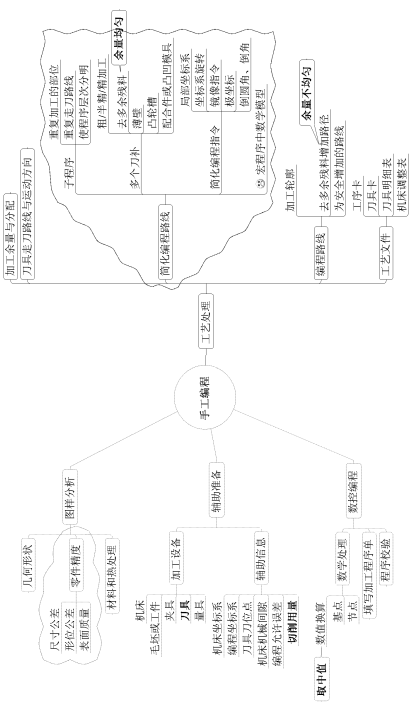
\includegraphics{images/图片1} 
	\caption{手工编程思维导图}\label{手工编程思维导图}
\end{figure}

\subsubsection{数控机床的操作}
如下面的思维导图 \ref{数控机床的操作思维导}
\begin{figure}	
	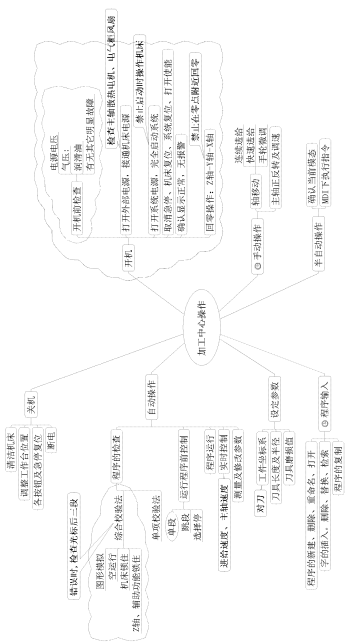
\includegraphics{images/图片2} 
	\caption{数控机床的操作思维导图} \label{数控机床的操作思维导}
\end{figure}

\subsubsection{数控机床指令}
\paragraph{G指令}\begin{itemize}
	\item G0 G1 G2 G3

	\item G17 G18 G19

	\item G9 G61 G62 G63 G64

	\item G4 \marginpar{说明介绍说明介绍说明介绍说明介绍说明介绍说明介绍}

	\item G20 G21

	\item G40 G41 G42 

	\item G43 G44 G49 \marginpar{说明介绍说明介绍说明介绍说明介绍说明介绍说明介绍}

	\item G90 G91

	\item G98 G99

	\item G81 G82 G83 G84 G85 G86 G87 G88 G89 G80 G73 G74 G76

\end{itemize}

\paragraph{M指令}

\begin{itemize}
	\item M0 M1 M2 M30

	\item M3 M4 M5 M19 

	\item M6 M7 M8 M9

	\item M98 M99

\end{itemize}

\paragraph{其它指令}
\subsubsection{常见加工结构}
\begin{itemize}
	\item 平面

	\item 外轮廓

	\item (岛屿)

	\item 孔
	\item 凸轮槽

	\item 复杂零件

	\item 配合零件

	\item CAD/CAM

	\item 宏程序

	\item 其它
\end{itemize}
\subsubsection{上学期期末试卷分析}
\subsection{课堂小结}
主要复习了数控方面的基本知识。
\vfill
\subsection{布置作业}
\begin{enumerate}[1、]
	\item 自选一零件图, 写出其工艺与程序;

	\item 写出如图所示零件的程序及与工艺;
\end{enumerate}


\jxhj{%教学后记
	}
\skrq{%授课日期
	}
\ktmq{%课题名称
	学习新内容 }
\jxmb{%教学目标,每行前面要加 \item
	\item 巩固上期的基本指令;

	\item 总结上期的编程思路;

	\item 总结机床的操作技巧;

	\item 了解本期的学习内容及学生情况;}
\jxzd{%教学重点,每行前面要加 \item
	\item 巩固上期的基本指令;

	\item 总结上期的编程思路;}
\jxnd{%教学难点,每行前面要加 \item
	\item 总结上期的编程思路;}
\jjff{%教学方法
	通过讲述、举例、演示法来说明;}

\makeshouye %制作教案首页

%%%%教学内容
\subsection{组织教学}
\begin{enumerate}[\hspace{2em}1、]
	\item 集中学生注意力;
	\item 清查学生人数;
	\item 维持课堂纪律;
\end{enumerate}
\subsection{复习导入及主要内容}
\begin{enumerate}[\hspace{2em}1、]
	\item 上学期末考试讲评;

	\item 了解学生情况;
\end{enumerate}
\subsection{教学内容及过程}
\subsubsection{本期教学安排} \marginpar{说明介绍}
\paragraph{理论教学计划:}
\begin{itemize}
	\item 复习上期内容

	\item 两面加工实例

	\item 变量与基本运算

	\item 椭圆加工if  goto

	\item 循环及其指令 if goto while

	\item 循环应用

	\item Siemens参数编程概述

	\item Siemens应用

	\item 镜象指令的使用

	\item 薄壁及配合件加工工艺

	\item 双曲线、抛物线加工

	\item 孔系加工(循环嵌套)

	\item 圆孔的宏程序

	\item 方槽椭圆槽的宏程序
	\item 斜面与圆柱面的宏程序

	\item 球面的宏程序(凸/凹)

	\item 椭球面的宏程序

	\item 任意轮廓倒圆角(系统变量)

	\item 任意轮廓倒圆角(G10)

	\item Siemens上倒角与倒圆

	\item 宏程序调用基本知识

	\item 宏程序调用的应用

	\item 多轴加工概述

	\item 四轴加工:圆柱凸轮的加工

	\item 五轴加工简介

	\item 综合练习(一)

	\item 综合练习(二)

	\item 综合练习(三)

	\item 综合练习(四)

\end{itemize}

\subparagraph{实习教学计划}
\begin{itemize}
	\item 两面加工类零件加工

	\item 薄壁配合件加工

	\item 宏程序加工

	\item 综合加工(钢材)
\end{itemize}

\subsubsection{手工编程复习} \marginpar{互动提问}
如下面的思维导图 \ref{手工编程思维导图}
\begin{figure}	
	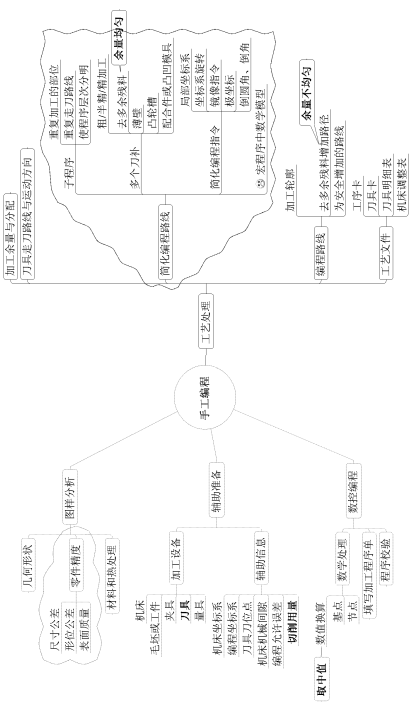
\includegraphics{images/图片1} 
	\caption{手工编程思维导图}\label{手工编程思维导图}
\end{figure}

\subsubsection{数控机床的操作}
如下面的思维导图 \ref{数控机床的操作思维导}
\begin{figure}	
	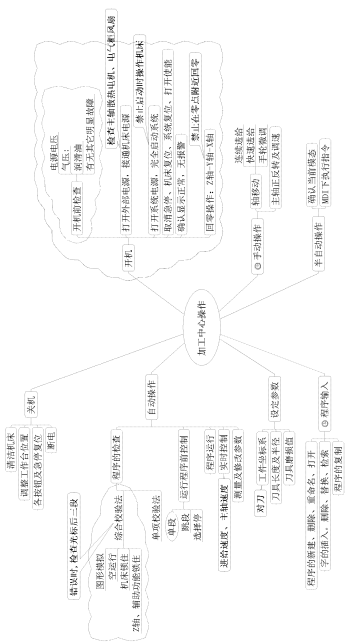
\includegraphics{images/图片2} 
	\caption{数控机床的操作思维导图} \label{数控机床的操作思维导}
\end{figure}

\subsubsection{数控机床指令}
\paragraph{G指令}\begin{itemize}
	\item G0 G1 G2 G3

	\item G17 G18 G19

	\item G9 G61 G62 G63 G64

	\item G4 

	\item G20 G21

	\item G40 G41 G42 

	\item G43 G44 G49

	\item G90 G91

	\item G98 G99

	\item G81 G82 G83 G84 G85 G86 G87 G88 G89 G80 G73 G74 G76

\end{itemize}

\paragraph{M指令}

\begin{itemize}
	\item M0 M1 M2 M30

	\item M3 M4 M5 M19

	\item M6 M7 M8 M9

	\item M98 M99

\end{itemize}

\paragraph{其它指令}
\subsubsection{常见加工结构}
\begin{itemize}
	\item 平面

	\item 外轮廓

	\item (岛屿)

	\item 孔
	\item 凸轮槽

	\item 复杂零件

	\item 配合零件

	\item CAD/CAM

	\item 宏程序

	\item 其它
\end{itemize}
\subsubsection{上学期期末试卷分析}
\subsection{课堂小结}
主要复习了数控方面的基本知识。
\vfill
\subsection{布置作业}
\begin{enumerate}[1、]
	\item 自选一零件图, 写出其工艺与程序.

	\item 写出如图所示零件的程序及与工艺.
\end{enumerate}


%% 中文习惯是设定首行缩进为2em。注意此设置一定要在document环境之中,这可能与\setlength作用范围相关
%\setlength{\parindent}{2em}                    
%
%\title{Xecjk Template Test}
%\author{Xiao Hanyu}
%\maketitle
%
%\tableofcontents
%\listoffigures
%%\listoftablescontent
%
%\section{基本文字测试}
\label{sec:1}
我叫肖晗宇,来自浙江大学计算机学院,热爱开源软件、旅行、摄影,推崇互助共享的精神理念。

My name is Xiao Hanyu, a student from Computer Science and Technology of Zhejiang University, I love open source software, travelling all over the world, photography, and so on. 

我喜欢\LaTeXe,也推荐大家来学习使用\LaTeXe,以下是比较不错的学习资源:

\begin{enumerate}
\item LaTeX companion
\item The TeXbook
\end{enumerate}


\section{图形图像测试}
\subsection{插图测试}
Hand in Hand:\ref{fig:hand_in_hand}
\begin{figure}[htbp]
\centerline{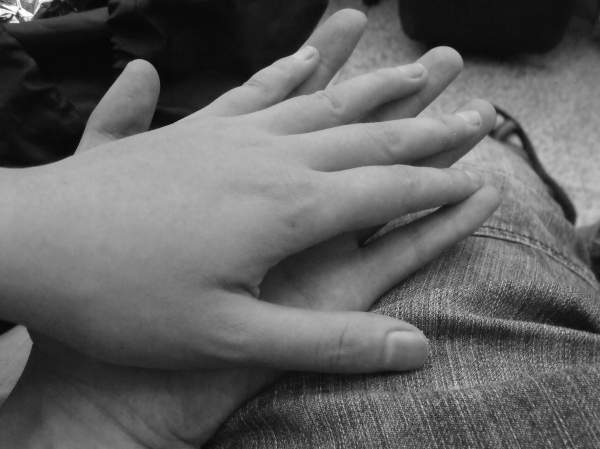
\includegraphics[width=0.6\textwidth]{images/hand_in_hand.png}}
\caption[]{\label{fig:hand_in_hand} 手拉手}
\end{figure}

\subsection{pgf/tikz绘图测试}
图\ref{fig:monotonic_chain}是用pgf/tikz宏包作的图形,用以说明计算几何相关定理。

\begin{figure}
\centering
\begin{tikzpicture}[line width=2pt]
\draw (-1,0) -- (8,0);
\draw (0,-1) -- (0,8);
\draw[step=.5cm, very thin] (0,0) grid (7.2,7.2);

\coordinate [label=above:$A$] (A) at (1, 4);
\coordinate [label=left:$B$] (B) at (0.5, 3.5);
\coordinate [label=left:$C$] (C) at (1, 3);
\coordinate [label=left:$D$] (D) at (0.3, 1.3);
\coordinate [label=below:$E$] (E) at (1, 1);

\draw[blue] (A) -- (B) -- (C)  -- (D) -- (E);
\draw[blue] (2, 0) -- (2, 6);

\coordinate [label=right:$A'$] (A') at (2, 4);
\coordinate [label=right:$B'$] (B') at (2, 3.5);
\coordinate [label=right:$C'$] (C') at (2, 3);
\coordinate [label=right:$D'$] (D') at (2, 1.3);
\coordinate [label=right:$E'$] (E') at (2, 1);

\draw[blue] (A) -- (A');
\draw[blue] (B) -- (B');
\draw[blue] (C) -- (C');
\draw[blue] (D) -- (D');
\draw[blue] (E) -- (E');

\coordinate [label=above:$a$] (a) at (5, 4);
\coordinate [label=left:$b$] (b) at (4.5, 4.5);
\coordinate [label=left:$c$] (c) at (5, 3);
\coordinate [label=left:$d$] (d) at (4.3, 1.3);
\coordinate [label=below:$e$] (e) at (5, 1.3);

\draw[green] (a) -- (b) -- (c)  -- (d) -- (e);
\draw[green] (6, 0) -- (6, 6);

\coordinate [label=right:$a'$] (a') at (6, 4);
\coordinate [label=right:$b'$] (b') at (6, 4.5);
\coordinate [label=right:$c'$] (c') at (6, 3);
\coordinate [label=right:$d'$] (d') at (6, 1.3);
\coordinate [label=right:$e'$] (e') at (6, 1.3);

\draw[green] (a) -- (a');
\draw[green] (b) -- (b');
\draw[green] (c) -- (c');
\draw[green] (d) -- (d');
\draw[green] (e) -- (e');
\end{tikzpicture}
\caption{Monotonic polygonal chains}
\label{fig:monotonic_chain}
\end{figure}

\section{表格测试}
\begin{table}[htbp]
  \centering
  \begin{tabular}[htbp]{r|l}
    \toprule
    日期 & 任务 \\
    \midrule
    2011.5 & 完善此份文档 \\
    2011.6 & 完善安装脚本 \\
    \bottomrule
  \end{tabular}
  \caption{表格}
  \label{tab:table1}
\end{table}

\section{源代码高亮测试}

以下是\href{http://acm.zju.edu.cn/onlinejudge/showProblem.do?problemCode=1372}{ZOJ 1372}的解题c++代码:

\begin{lstlisting}[language=c++]
#include <iostream>
#include <string>
using namespace std;
 
const long max_points = 100;
const long infinity = 1000001;
 
int p, r, length, g[max_points][max_points];
bool flag;
 
class vertex
{
public:
    int distance;
    bool visited;
};
 
vertex v[max_points];
 
void initial()
{
    for(int i = 1; i <= p; i++)
        for(int j = 1; j <= p; j++)
            g[i][j] = infinity;
}
 
void prim(int origin)
{
    int temp_min;
    int temp_v = 0;
    int sum = 0;
 
    for(int i = 1; i <= p; i++)
    {
        v[i].distance = g[i][origin];
        v[i].visited = false;
    }
 
    v[origin].distance = 0;
    v[origin].visited = true;
 
    sum++;
 
    while (sum < p)
    {
        temp_min = infinity;
        for(int i = 1; i <= p; i++)
            if(v[i].visited == false && v[i].distance < temp_min)
            {
                temp_min = v[i].distance;
                temp_v = i;
            }
         
        if(temp_min < infinity)
        {
            length += v[temp_v].distance;
            v[temp_v].visited = true;
            sum++;
        }
        else
        {
            flag = true;
            break;
        }
 
        for(int i = 1; i <= p; i++)
        {
            if(v[i].visited == false && v[i].distance > g[i][temp_v])
            {
                v[i].distance = g[i][temp_v];
            }
        }
    }
}
 
int main(int argc, char *argv[])
{
    int a, b, c;
 
    while(cin >> p)
    {
        if(p == 0)
            break;
        cin >> r;
 
        initial();
 
        for(int i = 0; i < r; i++)
        {
            cin >> a >> b >> c;
            if(c < g[a][b])
                g[a][b] = g[b][a] = c;
        }
        length = 0;
        prim(1);
 
        cout << length << endl;
    }
 
    return 0;
} 
\end{lstlisting}

\section{数学公式测试}

著名的爱因斯坦质能方程(\ref{eq:emc2}):

\begin{equation}
  \label{eq:emc2}
  E=mc^2
\end{equation}

计算$f(x)=x^2$的不定积分(\ref{eq:2}):

\begin{equation}
  \label{eq:2}
  \int x^2 dx = \frac{1}{3} x^3
\end{equation}
\section{参考文件测试}
参考文件最好使用bibtex,关于bibtex的使用方法,你可以自行查阅相关文献。

这里是参考文献\cite{c_minigui}

%%%%%%%%%------------------------------------------------------------------------
%%%% 附录

% \appendix    
% \appendixpage
%% 将附录条目添加到contents
% \addappheadtotoc

%%%% 附录结束
%%%%%%%%------------------------------------------------------------------------

%
%%% 加入参考文献支持
%\bibliography{data/main}
%%% 解决目录中没有相应的参考文献的条目问题
%\addcontentsline{toc}{section}{\refname} 
\end{document}
%%%% 正文部分结束
%%%%%%%%------------------------------------------------------------------------
